\subsection{Encoding/Decoding}

\begin{frame}{Encoding/Decoding - NNs}
	\begin{itemize}[\textbullet]
		\item \textbf{Decoding :} Implicit neural representation.
		\begin{equation*}
			u_\theta(x)=\mathcal{D}_{\theta_u}(x)=u_{NN}(x)
		\end{equation*}
		with $u_{NN}$ a neural network (for example a MLP). \\
		$\Rightarrow$ non-linear decoding $\Rightarrow$ approximation space $V_N$ = finite-dimensional variety \\
		$\Rightarrow$ there is no unique projector
		\item \textbf{Encoding :} Optimization process.
		\begin{equation*}
			\theta_f=E(f)=\arg\min_{\theta\in\mathbb{R}^N}\int_\Omega ||f_\theta(x)-f(x)||^2 dx
		\end{equation*}
	\end{itemize}
\end{frame}

\begin{frame}{Neural Network Decoder}
	\textbf{Advantages of a non-linear decoder :}
	\begin{itemize}[\textbullet]
		\item We gain in the richness of the approximation
		\item We can hope to significantly reduce the number of degrees of freedom
		\item This avoids the need to use meshes. \\ \; \\
		
		\begin{center}
			\begin{minipage}{0.4\linewidth}
				polynomial models \\
				$\Rightarrow$ local precision \\
				$\Rightarrow$ use meshes \\ \; \\
				\centering
				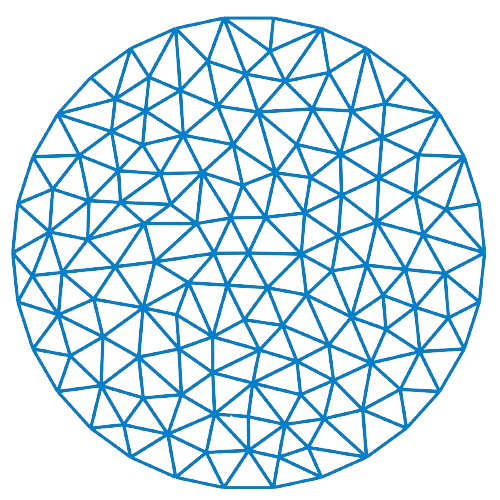
\includegraphics[width=0.6\linewidth]{images/pinns/nonlineardecoder_mesh.png}
			\end{minipage} \quad \vline \quad
			\begin{minipage}{0.4\linewidth}
				NN models \\
				$\Rightarrow$ global precision \\
				$\Rightarrow$ no need to use meshes \\ \; \\
				\centering
				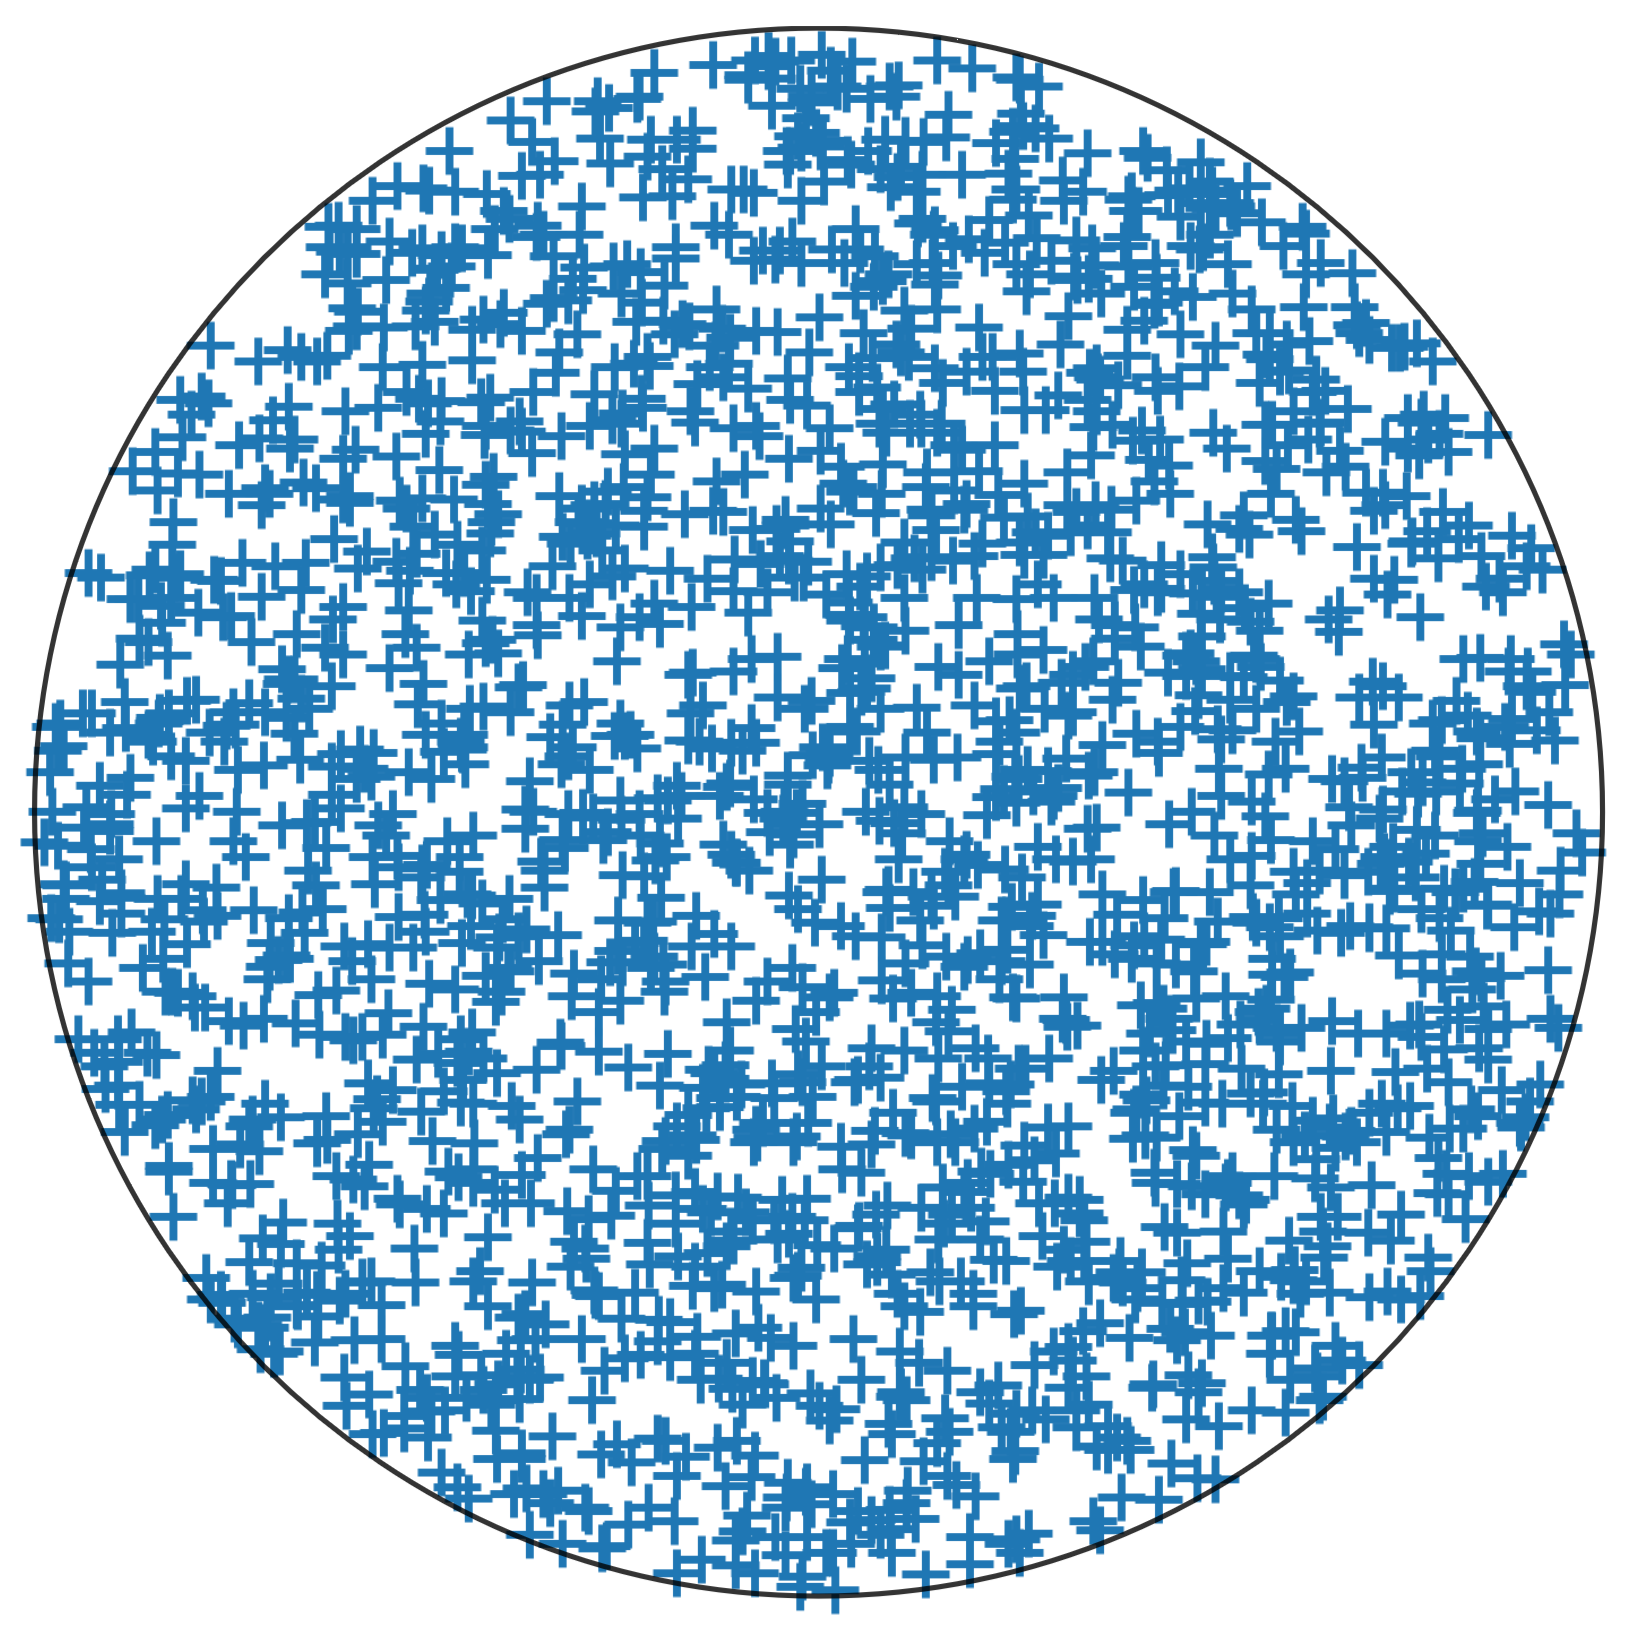
\includegraphics[width=0.6\linewidth]{images/pinns/nonlineardecoder_random.png}
			\end{minipage}
		\end{center}
	\end{itemize}
\end{frame}

\subsection{Approximation}

\begin{frame}{Approximation}
	\textbf{Idea :} Project a certain form of the equation onto the variety $\mathcal{M}_N$. \\
	
	\vspace{10pt}
	
	\textbf{Discretization :} Degrees of freedom problem (no mesh).
	\begin{center}
		$u=\arg\min_{v\in \mathcal{M}_N} J(v) \quad \longrightarrow \quad \theta_u=\arg\min_{\theta\in \mathbb{R}^N} J(\theta) $
	\end{center}
	with $J$ a functional to minimize.
	
	\vspace{10pt}
	
	\textbf{Variants :} Depends on the problem form used for projection.
	
	\begin{center}
		\begin{tabular}{c|c}
			\textbf{Symmetric spatial PDE} & \textbf{Any type of PDE} \\
			Problem - Energetic form & Problem - Least-square form \\
			Deep-Ritz & Standard PINNs \\
			(Galerkin projection) & (Galerkin Least-square projection)
		\end{tabular}
	\end{center}
\end{frame}

\begin{frame}{Deep-Ritz}
	\small 
	\textbf{Discrete minimization Problem :} Considering the energetic form of our PDE, our discrete problem is
	\begin{equation}
		\theta_u=\arg\min_{\theta\in\mathbb{R}^N} J_{in}(\theta)+J_{bc}(\theta) \label{minpb_deepritz}
	\end{equation}
	with 
	\begin{equation*}
		J_{in}(\theta)=\frac{1}{2}\int_\Omega L(v_\theta)v_\theta - \int_\Omega fv_\theta  \qquad \text{and} \qquad J_{bc}(\theta)=\frac{1}{2}\int_{\partial\Omega} (v_\theta-g)^2
	\end{equation*}	
	
	\textbf{Monte-Carlo method :} Discretize the cost function by random process.
	
	\begin{itemize}[\textbullet]
		\item $(x_1,\dots,x_n)$ randomly drawn according to $\mu(x)$ defined on $\Omega$ 
		\begin{equation*}
			J_{in}(\theta)=\frac{1}{2n}\sum_{i=1}^n L(v_\theta(x_i))v_\theta(x_i) - \frac{1}{n}\sum_{i=1}^n f(x_i)v_\theta(x_i)
		\end{equation*}
		\item $(y_1,\dots,y_{n_b})$ randomly drawn according to $\mu_b(x)$ defined on $\partial\Omega$
		\begin{equation*}
			J_{bc}(\theta)=\frac{1}{2n_b}\sum_{i=1}^{n_b} (v_\theta(y_i)-g(y_i))^2
		\end{equation*}
	\end{itemize}	

	\footnotesize
	\textit{Remark :} \ding{217} Two different random generation processes (to have enough boundary points) \\
	\ding{217} Weights in front of the cost functions still need to be determined
\end{frame}

\begin{frame}{Standard PINNs}
	\textbf{Discrete minimization Problem :} Considering the least-square form of our PDE, our discrete problem is
	\begin{equation}
		\theta_u=\arg\min_{\theta\in\mathbb{R}^N} J_{in}(\theta)+J_{bc}(\theta) \label{minpb_pinns}
	\end{equation}
	with 
	\begin{equation*}
		J_{in}(\theta)=\frac{1}{2}\int_\Omega (L(v_\theta) - f)^2  \qquad \text{and} \qquad J_{bc}(\theta)=\frac{1}{2}\int_{\partial\Omega} (v_\theta-g)^2
	\end{equation*}	
	
	\textbf{Monte-Carlo method :} Discretize the cost function by random process.
	
	\begin{itemize}[\textbullet]
		\item $(x_1,\dots,x_n)$ randomly drawn according to $\mu(x)$ defined on $\Omega$ 
		\begin{equation*}
			J_{in}(\theta)=\frac{1}{2n}\sum_{i=1}^n (L(v_\theta(x_i)) - f(x_i)))^2
		\end{equation*}
		\item $(y_1,\dots,y_{n_b})$ randomly drawn according to $\mu_b(x)$ defined on $\partial\Omega$
		\begin{equation*}
			J_{bc}(\theta)=\frac{1}{2n_b}\sum_{i=1}^{n_b} (v_\theta(y_i)-g(y_i))^2
		\end{equation*}
	\end{itemize}	

	\footnotesize
	\textit{Remark :} Same.
\end{frame}

\begin{frame}{In practice...}
	\begin{itemize}[\ding{217}]		
		\item Use regular model, derivable several times (and automatic differentiation)
		
		\item Activation functions regular enough to be derived 2 times (due to the Laplacian) \\
		$\Rightarrow$ Tangent Hyperbolic rather than ReLU \\
		(or adaptive methods where we parameterize the activation functions)
		
		\begin{center}
			\begin{minipage}{0.43\linewidth}
				\raggedleft
				\pgfimage[width=0.6\linewidth]{images/pinns/relu.png}
			\end{minipage} \hfill
			\begin{minipage}{0.1\linewidth}
				\centering
				\pgfimage[width=\linewidth]{images/pinns/fleche.png} 
			\end{minipage} \hfill
			\begin{minipage}{0.43\linewidth}
				\raggedright
				\pgfimage[width=0.65\linewidth]{images/pinns/tanh.png}
			\end{minipage}
		\end{center}
	
		\item Stochastic gradient descent method (by mini-batch) - ADAM method \refappendix{frame:adam}		
	\end{itemize}

	\textbf{To go further :}
	\begin{itemize}[\ding{217}]				
		\item Standard PINNs : possibility of adding a $J_{data}$ cost function \\
		$\rightarrow$ to approximate already known solutions
		
		\item Impose boundary conditions using a LevelSet function
	\end{itemize}

	
\end{frame}

\begin{frame}{Steps Decomposition - NNs}
	\vspace{10pt}
	\small
	\renewcommand{\arraystretch}{1.3}
	\begin{tabular}{|c|c|c|c|}
		\hline
		\textbf{Encoding} & \multicolumn{2}{c|}{\textbf{Approximation}} & \textbf{Decoding} \\
		\hline
		$f \; \rightarrow \theta_f$ & \multicolumn{2}{c|}{$\theta_f \; \rightarrow \theta_u$} & $\theta_u \; \rightarrow u_\theta$ \\
		\hline
		\multicolumn{4}{c}{ } \\
		\hline
		\multicolumn{4}{|c|}{\textbf{Mesh-based Methods}} \\
		\hline
		\multirow{3}{*}{$\begin{aligned}
				\theta_f&=\mathcal{E}(f) \\
				&=M^{-1}b(f)
			\end{aligned}$} & Galerkin & LS Galerkin & \multirow{3}{*}{$\begin{aligned}
				u_\theta(x)&=\mathcal{D}_\theta(x) \\
				&=\sum_{i=1}^N (\theta_u)_i\varphi_i
			\end{aligned}$} \\
		 & \footnotesize $\langle R(u_\theta),\varphi_i\rangle=0$ & \footnotesize $\langle R(u_\theta),(\nabla_\theta R(u_\theta))_i\rangle=0$ & \\
		\cline{2-3}
		 & \multicolumn{2}{c|}{$A\theta_u=B$} & \\
		\hline
		\multicolumn{4}{c}{ } \\
		\hline
		\multicolumn{4}{|c|}{\textbf{Physically informed learning}} \\
		\hline
		\multirow{3}{*}{\footnotesize $\displaystyle\theta_f=\min_{\theta\in\mathbb{R}^N} \int_\Omega ||f_\theta-f||^2$} & Deep-Ritz & Standard PINNs & \multirow{3}{*}{$u_\theta(x)=u_{NN}(x)$} \\
		 & \footnotesize Energetic Form & \footnotesize LS Form & \\
		\cline{2-3}
		 & \multicolumn{2}{c|}{$\theta_u=\arg\min_{\theta\in \mathbb{R}^N} J(\theta)$} & \\
		\hline
	\end{tabular}
\end{frame}

